% !TEX root = main.tex

\section{传输层} % transport layer
传输层协议称为\textbf{端到端}或\textbf{进程到进程}的协议。 因特网的传输层可以为两个进程在\textbf{不可靠的网络层}上建立一条\textbf{可靠的逻辑链路},可以提供\textbf{字节流}传输服务,并且可以进行\textbf{流控制}和\textbf{拥塞控制}。

因特网的传输层有两个协议: UDP和TCP。
UDP协议提供不可靠的尽力服务, TCP协议提供可靠的字节流服务。
协议号:TCP为6,ICMP=1;UDP为17,IGMP=2

TCP/UDP通过数据段(segment)中的目的端口号(2B)确定将收到的数据段交给上层哪个进程。
\begin{itemize}
    \item 知名端口:0-1023,为提供知名网络服务的系统进程所用。    例如: 80-HTTP, 21-ftp Control, 20-ftp Data, 23-telnet,25-SMTP, 110-POP3,53-DNS
    \item 注册端口:1024-49151。在IANA注册的专用端口号,为企业软件所用。
    \item 动态端口:49152-65535,没有规定用途的端口号,一般用户可以随意使用。也称为私    用或暂用端口号。
\end{itemize}

\subsection{UDP协议}
用户数据报协议(User Datagram Protocol, UDP)只提供\textbf{无连接的不可靠的尽力服务}。发送给接收进程的数据有可能丢失,也有可能错序。
可以说UDP协议是IP协议的简单扩展,在IP协议上增加了\textbf{端口号},把进程关联起来了。

接收进程每次接收一个完整的数据报,如果进程设置的接收缓冲区不够大,收到的数据报将被截断。

数据报的内容
\begin{itemize}
    \item 总长度:整个UDP报文长度
    \item 源端口号和目的端口号:用于关联发送进程和接收进程
    \item 校验和:由\textbf{伪IP头(就是用来算校验和用)}、 UDP头(校验和为0)和UDP数据形成。其中,伪IP头的协议号为17。如果发送方把校验和设置为0,接收方会忽略校验和。 UDP长度就是UDP头部的总长度。
\end{itemize}


\subsection{TCP协议}
传输控制协议(Transmission Control Protocol, TCP)为进程之间提供\textbf{面向连接的可靠的}数据传送服务(通过滑动窗口协议实现)。TCP为\textbf{全双工}协议。TCP提供\textbf{流控制}机制,即控制发送方的发送速度,使发送的数据不会淹没接收方。作为因特网的主要数据发源地,TCP还提供\textbf{拥塞控制}功能。
\begin{figure}[H]
    \centering
    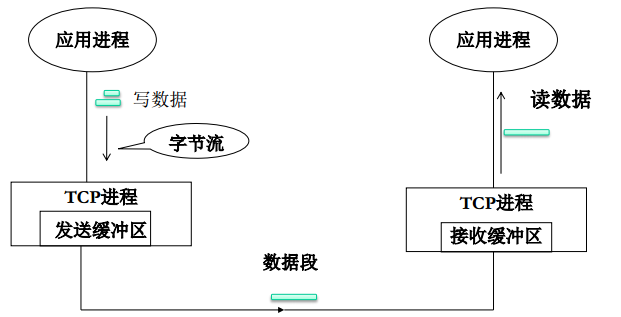
\includegraphics[width=0.5\linewidth]{fig/TCP.PNG}
\end{figure}

\begin{itemize}
\item 一个TCP连接提供\textbf{可靠的字节流服务}。字节流服务表示\textbf{没有消息边界}。例如,多次发送的数据可以放在一个数据段中传送且\textbf{不标识边界}。
\item 每个数据段的数据部分的最大长度(字节)不能超过MSS(Maximum Segment Size)。
\item 每个TCP连接可以由四元组唯一标识:\underline{源IP地址、源端口号、目的IP地址、目的端口号},通过\textbf{端口号}区分不同进程。
\item 客户端通过查路由表知道\textbf{IP地址},\textbf{端口号}自动选一个未用的
\end{itemize}

TCP数据报格式:头部长度以四个字节为单位。校验和由伪IP头、 TCP头和TCP数据部分形成。其形成方法与UDP协议类似。
字节流中的每个字节均被编号。初始序号采用基于时间的方案, 一般采用随机数。
数据部分的第一个字节的编号为初始序号加1。
\begin{itemize}
\item SYN:表示建立连接
\item FIN:表示关闭连接,不再发送数据,但是可以接收数据,也可以发送\textbf{数据段}(不包含数据)
\item ACK:表示响应
\item PSH:将接收缓冲区的进程全部推给接收方进程
\item RST:发现连接可能出了问题,连接重置
\item URG:紧急指针用于指出紧急/带外数据(out-of-band)的边界,紧急数据最后一个字节
\end{itemize}

TCP协议工作过程
\begin{center}
    \begin{tikzcd}
        \text{建立连接}\arrow{r} & \text{传送数据} & \text{释放连接}
    \end{tikzcd}
\end{center}
\begin{itemize}
    \item 建立连接:非对称活动,服务器一直在等,客户向服务器呼叫
    \item 传送数据:全双工方式
    \item 释放连接:对称活动,可由任何一方发起
\end{itemize}

三次握手建立连接:x,y为初始序号,随机数
\begin{itemize}
    \item SYN,Seq\#=x
    \item (Client)SYN+ACK,Seq\#=y; Ack\#=x+1
    \item ACK,Ack\#=y+1
\end{itemize}
这里确认号含义与数据链路层不同,这里是\textcolor{red}{\textbf{期待接收}}的序号

四次握手关闭连接
\begin{itemize}
    \item FIN,Seq\#=x
    \item (Client)ACK,Ack\#=x+1
    \item (Client)FIN,Seq\#=y
    \item ACK,Ack\#=y+1
\end{itemize}
可以合并中间两次握手(ACK和FIN)或两方同时发出ACK

先发送FIN报文的一方在ACK发送完毕后需要等待2MSL(Maximum Segment Lifetime)的时间才\textbf{完全关闭}连接(占用端口号)。 TCP标准中MSL采用60秒, Unix采用30秒。\textbf{避免通道中还有未到达的数据}。
\begin{figure}[H]
    \centering
    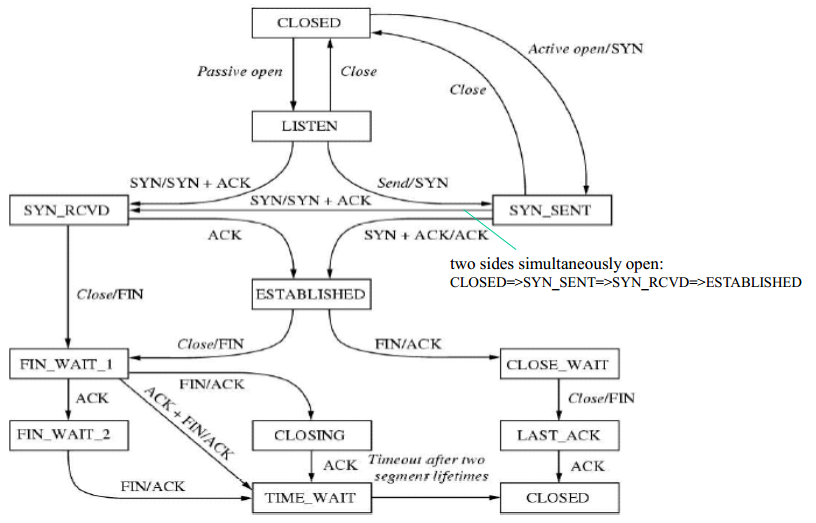
\includegraphics[width=0.8\linewidth]{fig/TCP-transition.PNG}
\end{figure}

TCP协议使用\textbf{选择性确认}协议,不使用NAK。只有\textbf{一个超时定时器}。
\begin{itemize}
\item 采用字节流方式,每个数据段使用其\textbf{第一个字节}的编号作为序号\footnote{数据链路层每一个帧占一个序号},按\textbf{字节}编号。
\item 确认号为\textbf{期待接收}\footnote{区别于数据链路层的滑动窗口,确认号是当前接收并确认的序号}的下一个\textbf{字节}(下一个数据段)的序号。
\item 由于TCP是对IP数据报的封装,要获取数据的长度,可以通过IP数据报中的总长度获取。
\item TCP协议没有说明如何处理错序到达的数据段,要取决于具体实现。
\end{itemize}

\begin{figure}[H]
    \centering
    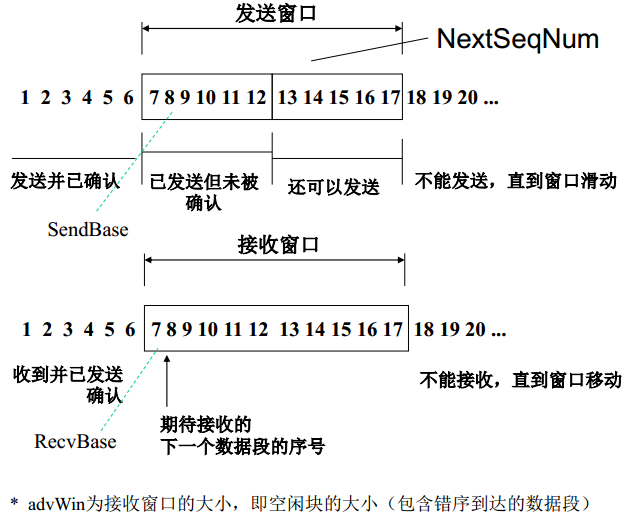
\includegraphics[width=0.8\linewidth]{fig/TCP-window.PNG}
\end{figure}

\begin{itemize}
\item 接收方先传MSS,x和接收窗口大小(advWin)
\item 发送方做发送窗口,序号为x+1,大小等同advWin大小(发送窗口大小是会变的)
\item 接收窗口大小\textbf{会变},不同于数据链路层;同理发送窗口大小\textbf{也会改变},用接收窗口大小设置发送窗口大小
\item 要等接收方进程将缓冲区取空,发送方才能继续发,否则发送窗口大小始终为0
\item 会自动移动超时定时器
\item 一旦发现有问题,立即减慢
\item 要考虑错序到达的数据段
\end{itemize}

数据链路层每个帧都有一个超时定时器,而传输层只有一个超时定时器。

\begin{itemize}
\item 如果发送方收到一个数据段的\textbf{3次重复的ACK}(包括第一次则一共4次),它就认为其后的数据段(由确认号指出) 已经丢失,在超时之前会重传该数据段,这种方法称为\textbf{快速重传}(fast retransmit)。
缺点是丢包时间很长,优点是可以减缓网络压力。
\item 采用\textbf{延迟确认}(delayed ACK)时,接收方并不在收到数据段立即进行确认,而是延迟一段时间再确认。如果这个期间收到多个数据段,则只需要发送一个确认。如果在这个期间接收方有数据帧要发往发送方,还可以使用捎带确认(piggybacking)。
大部分的系统(Windows/Unix)的延迟确认时间为200毫秒。TCP标准要求延迟确认不大于500毫秒。
\item \textbf{选择性确认}允许接收方把收到的数据块通过数据段的选项告知发送方,使发送方不会重传这些数据块
\end{itemize}

Go back N超时重传1个RTT,没有中间结点,故可以用固定的超时时间。
但由于TCP涉及多个结点,故需要实时变化,进行估计。

总结传输层滑动窗口协议和数据链路层的区别
\begin{center}
\begin{tabular}{|c|c|c|}\hline
     & 传输层 & 数据链路层\\\hline
    序号 & 随机初始序号+1,按字节计数 & 每一个帧一个序号 \\\hline
    确认号 & 期待接收的序号 & 收到哪一个就用哪一个,代表当前与之前的全收到了\\\hline
超时定时器 & \begin{tabular}{c}只有一个,只要有未确认的数据段\\就会启动(针对未确认序号最小的);超时没收到确认,就会重传\end{tabular} & 每个帧都有一个\\\hline
\end{tabular}
\end{center}

原始公式
\[\text{EstimatedRTT} = (1-\alpha)\times \text{EstimatedRTT} + \alpha \times \text{SampleRTT}\]
\begin{itemize}
    \item $0<\alpha<1$, $\alpha$越小过去样本的影响越大。
    \item 一般取值$\alpha=0.9$,这会使过去影响指数减少。
    \item 这个公式也称为指数加权移动平均方法(Exponentially Weighted Moving Average, EWMA)
    \item $\text{RTO(retransmission timeout)} = 2\times \text{EstimatedRTT}$
\end{itemize}

TCP超时计算最常用的算法---Jacobson算法
\begin{itemize}
    \item 修改上一页公式的参数:$\alpha=1/8$。
    \item Jacobson/Karels提议RTO计算还要加上一个合适的安全边际(safety margin),使得在样本变化较大时RTO会很快变得更大。
\end{itemize}
\[\text{RTO} = \text{EstimatedRTT} + 4\times \text{DevRTT}\]
\[\text{DevRTT} =(1-\beta)\times\text{DevRTT} + \beta\times|SampleRTT-EstimatedRTT|\]
一般设$\beta = 1/4$

采样频率:如果发送窗口为12MSS,则每12个段取样一次。

Karn算法:在收到重传段确认时不要计算EstimatedRTT。在每次重传时直接把RTO加倍直到数据段首次得到确认,并把这个RTO作为后续段的RTO。这个修正称为Karn算法(Karn and Partridge, 1987)。每次收到非重传段的ACK之后,就计算EstimatedRTT和正常的RTO,并用这个RTO作为后续段的RTO。

在12次重传后TCP协议发送rst数据段并关闭连接。

\begin{itemize}
\item 流控制:单一发送方和接收方,控制发送的速度
\item 拥塞控制:大家都发数据,使整个网络的数据太多,让每一个都不要传那么快
\end{itemize}

拥塞简单来说“太多的主机发送太快太多的数据给网络处理”。这不同于流控制!表现为:
\begin{itemize}
    \item 丢包(路由器上缓冲区溢出)
    \item 长延迟(在路由器缓冲区中排队)
\end{itemize}
不主张发送ICMP包,加重拥塞;靠TCP自己发现拥塞。

拥塞控制的两大类方法:
\begin{enumerate}
    \item 端到端的拥塞控制:
\begin{itemize}
    \item 没有来自网络的明确的反馈
    \item 终端系统通过丢包和延迟推导的拥塞
    \item TCP协议的方法
\end{itemize}
    \item 网络辅助的拥塞控制:
\begin{itemize}
    \item 路由器反馈给终端系统
    \item 用一个比特指出拥塞发生(SNA, DECbit, TCP/IP ECN, ATM)
    \item 向发送方给一个明确的发送速率
\end{itemize}
\end{enumerate}

\begin{itemize}
    \item 超时或收到3个重复ack就认为丢包了,看作拥塞发生了
    \item TCP协议通过减少发送速率来控制拥塞。发送速率与发送窗口大小有关:
\[\text{发送速率 rate $=$ SWS(Sending Window Size)$/$RTT}\]
    \item 引入拥塞窗口变量CongWin来限制SWS。
\[SWS = \min(\text{CongWin}, \text{AdvWin})\]
CongWin发送窗口限制,Adcwin接收方要求的流量控制
    \item TCP协议改变CongWin的三种机制:
    \begin{itemize}
        \item 加性增乘性减(AIMD)
        \begin{figure}[H]
            \centering
            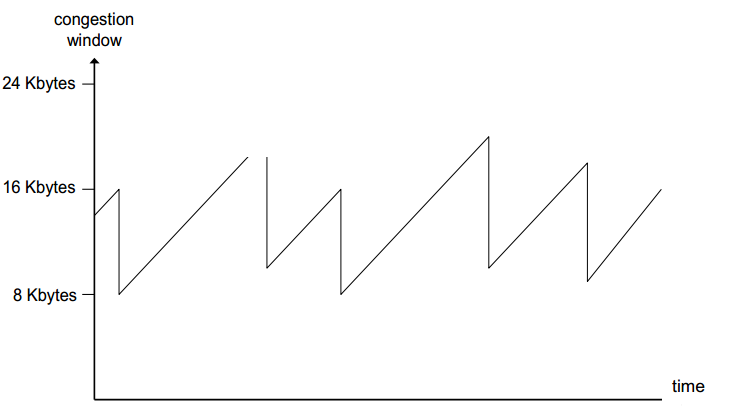
\includegraphics[width=0.6\linewidth]{fig/congression-AIMD.PNG}
        \end{figure}
        \item 慢启动(slow start)
        \begin{figure}[H]
            \centering
            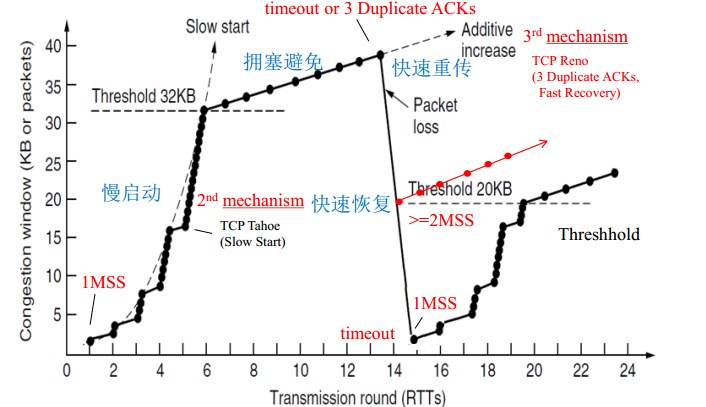
\includegraphics[width=0.6\linewidth]{fig/congression-slow-start.PNG}
        \end{figure}
        \begin{enumerate}
            \item 初始时, CongWin设为1 MSS, 阈值(threshold)设为65535, 发送一个数据段。
            \item 在当前窗口所有数据段的确认都收到之后, CongWin加倍。
            实际上,每收到一个确认, CongWin增加一个MSS。把它称为慢启动(slow start)是因为这个方法比立即采用通知窗口更慢。
            \item 当拥塞发生时,把当前CongWin (或SWS)的一般保存为阈值(threshold),然后CongWin又从 1MSS开始慢启动。
            \item 当 CongWin增长到等于或大于阈值(threshold)时,在当前窗口所有数据段的确认都收到之后, CongWin增加一个MSS。(Congestion Avoidance)实际上, 每收到一个ACK, CongWin增加SegSize*SegSize/CongWin。如果发生拥塞,转 (3)。
            \item 用系统参数TCP\_MaxWin(一般为65535)限制 CongWin的大小。
            \begin{itemize}
                \item SegSize 为被确认的数据段的大小
                \item 假设算法开始时通知窗口大小AdvWin=65535
            \end{itemize}
        \end{enumerate}
        \item 在超时时间之后的保守方法
    \end{itemize}
\end{itemize}

随机初始序号和2MSL都用于阻止重建TCP连接相同4元组,不会收到上一次连接遗留的数据的干扰

问题一---长肥管道:带宽大,未确认的数据量(capacity=bandwidth*RTT)
\begin{itemize}
\item \textbf{序号回绕}问题(因为速度太快):使用一般数据段的选项\verb'timestamp'(TS)。只用于区分回绕的序号是不同的,不用于确定先后次序。TS也用来测量RTT。
\[\text{Window Size} = \text{AdvertisedWindow} * 2\text{WinScale}\]
\item \textbf{发送窗口太小},满足不了要求:当丢包发生时,由于SWS的限制,管道将会被清空。解决方法:快速重传、快速恢复。(数据链路不会,因为直连网)
\end{itemize}

问题二---死锁现象:win为0,接收方取空,再发不为空的ACK丢失了。
缓冲区不变化,不会发确认回来
\begin{itemize}
\item 接收方可以启动一个超时定时器,可以是可以,但如果发送方没有数据传了,那接收方还是会继续发。(无谓发送数据)
\item 一般从发送方解决:在发送窗口为0之后,并且发送方有数据要发送,则启动坚持定时器(Persist Timer),定期从要发送的数据中取一个字节发送出去(Window Probe),直到收到不为0的通知窗口为止
\end{itemize}

问题三---傻瓜窗口症候(silly window syndrome)
\begin{itemize}
    \item 发送进程有很多小批量数据要发送,如用telnet作为远程终端:设个定时器,到时间就把缓冲区内容发送出去\\
    Nagle算法---启发式算法
    \begin{figure}[H]
        \centering
        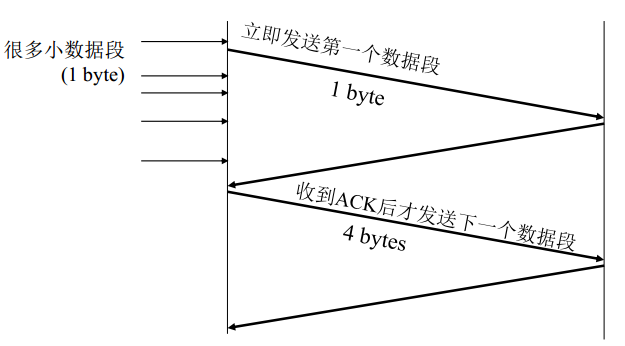
\includegraphics[width=0.6\linewidth]{fig/nagle.PNG}
    \end{figure}
    \begin{enumerate}
        \item 立即发送一个数据段,即使发送缓冲区只有一个字节
        \item 只有收到\underline{上一个数据段的确认}(此时缓冲区已经积累一定数据)或者\underline{发送缓冲区中数据超过MSS},才可以发送下一个数据段
        \item 对于即时性要求高的地方,如Window方式的鼠标操作,要\textbf{关闭}Nagle算法
    \end{enumerate}
    \item 接收方问题,接收进程频繁取走小批量数据\\
    Clark算法:当接收缓冲区的空闲块大小变得很小时,要等到空闲块大小为接收缓冲区大小的一半或达到 MSS时才发送确认。
\end{itemize}

TCP定时器
\begin{itemize}
\item 每个连接只针对第一个未确认数据段启动重传定时器(retransmission timer)。所有数据段都已确认,则关闭它。超时重传或发送窗口移动时要重启该定时器。
\item 持续定时器(persist timer)用于保持窗口大小信息流动即使连接的另一端关闭了接收窗口。
\item 保活定时器(keepalive timer)在\textbf{长时间}没有交换数据段之后,用于检测连接的另一端是否出了问题。(如微信)隔2个小时,发10个数据段,如果没有ACK则关闭连接。(由应用层程序来做而不是TCP)
\item 处于TIME\_WAIT状态的连接一方需要等待2MSL秒,时间到才能关闭连接。
\end{itemize}